\documentclass{beamer}
\usepackage{beamerthemesplit}
\usepackage{booktabs}
\usepackage{graphicx}
\usepackage{transparent}
\usepackage{bbold}
\usepackage[italian]{babel}
\usepackage[utf8x]{inputenc}
\usepackage{listings}
\usepackage{tikz}
\usetikzlibrary{fit, shapes, arrows, patterns, matrix}
\usepackage{amsmath,amsfonts,amssymb}
\usepackage{pgfplots}
\usepackage{scalefnt}
\usepackage{color}
\usepackage{xcolor}
\usepackage{multicol}
\usepackage{bm}
\usepackage{changepage}

\title[Algoritmi]{Algoritmi di feature selection}
\institute{
\begin{small}
Corso di Laurea in Informatica Magistrale
\end{small}}
\author{\textbf{Simone Rutigliano}}
\date{\tiny{\today}}

\usebackgroundtemplate{
%    \transparent{0.12}{
     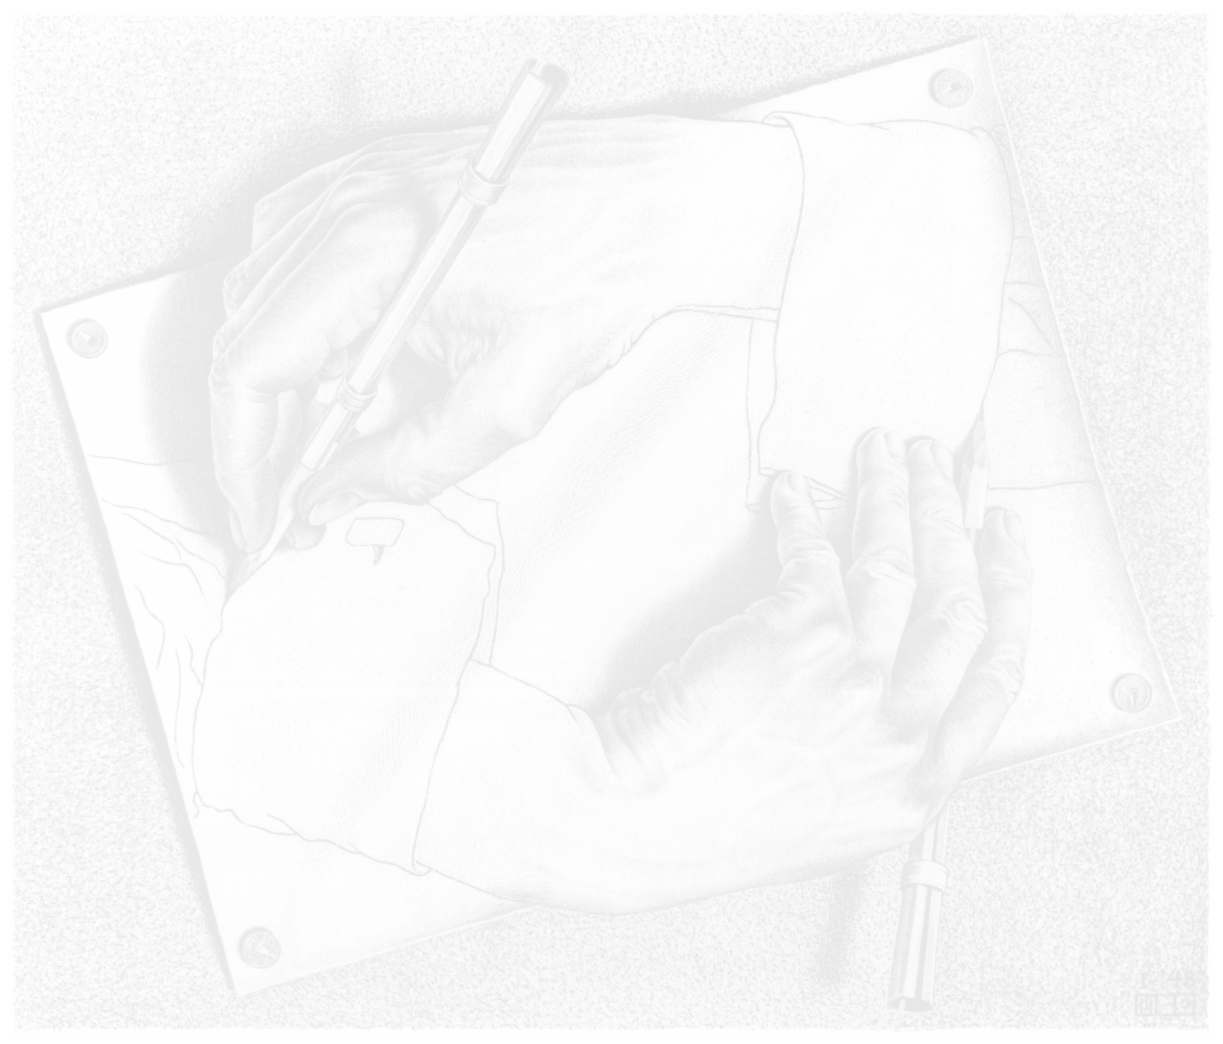
\includegraphics[width=\paperwidth, height=\paperheight]{./figure/theme/escher_hands_tr.png}
%    }
}

%\usetheme{Hannover}
\usetheme{Copenhagen}
\usecolortheme{seahorse}
\usecolortheme{rose}
%\usetheme{Frankfurt}
%\usecolortheme{beetle}

%\useoutertheme[subsection=false]{smoothbars}
%\useoutertheme[subsection=false]{smoothtree}
\useoutertheme{shadow}
\setbeamercovered{dynamic}

\pgfdeclareimage[height=1cm]{logo}{figure/theme/logo}
\logo{\pgfuseimage{logo}}

\begin{document}

%%%%%%%%%%%%%%%%%%%%%%%%%%%%%%%%%%%%%%%%%%%%%%%%%%%%%

\begin{frame}
\maketitle
\end{frame}

%%%%%%%%%%%%%%%%%%%%%%%%%%%%%%%%%%%%%%%%%%%%%%%%%%%%%

\begin{frame}
\frametitle{Outline}
	\begin{columns}
		\begin{column}{0.4\textwidth}
			\begin{equation*}
			\qquad \textbf{Java}
			\begin{cases} 
			PageRank
			\\ 
			HITS
			\\
			SALSA
			\\
			ReConRank
			\\
			SimRank
			\\
			TripleRank
			\\
			mRMR
			\\
			PICSS
			\end{cases}
			\end{equation*}
		\end{column}
		\begin{column}{0.8\textwidth}
			\begin{equation*}
			\qquad \textbf{RapidMiner}
			\begin{cases} 
			SHSEL \begin{cases} 
			Information ~Gain \\ \mbox{\emph{Correlation}}
			\end{cases}
			\\~\\
			Greedy Top Down
			\end{cases}
			\end{equation*}
		\end{column}
	\end{columns}
\end{frame}

\section{Algoritmi Java}
\subsection{PageRank}
\begin{frame}
	\frametitle{PageRank}
	Implementazione del \emph{Wrapper Model}: 
	\begin{itemize}
		\item Utilizzare lo stesso algoritmo sia per la feature selection sia per la fase di raccomandazione
		\item Subset ottimizzato per la raccomandazione
	\end{itemize}
\end{frame}
\subsection{HITS}
\begin{frame}
	\frametitle{HITS}
	Creazione del subset attraverso l'utilizzo dell'algoritmo di \emph{Hyperlink-Induced Topic Search} basato sul \emph{ranking} di risorse in base a due metriche:
	\begin{itemize}
		\item Hub
		\item Authority
	\end{itemize}
	Implementazioni trovate:
	\begin{itemize}
		\item \url{http://goo.gl/4pWAq4}
		\item \url{http://goo.gl/qSDXru}
	\end{itemize} 
\end{frame}
\subsection{SALSA}
\begin{frame}
	\frametitle{SALSA}
	\begin{itemize}
		\item Combinazione di HITS e PageRank
		\item Usa i punteggi di Hub e Autority
		\item Crea un grafo bipartito $G=(V_1 \cup V_2,E)$ dove \begin{itemize}
			\item $V_1$ rappresenta il set degli Hub
			\item $V_2$ rappresenta il set degli Autority
			\item Una risorsa può essere contenuta sia in un set che nell'altro
		\end{itemize}
	\end{itemize}
	Implementazione trovata:
	\begin{itemize}
	\item \url{http://goo.gl/DtHa4K}
	\end{itemize}
\end{frame}
\subsection{ReConRank}
\begin{frame}
	\frametitle{ReConRank}
	Tratto dal paper \cite{Hogan06reconrank:a}
	\begin{itemize}
	\item 	Basato su due ranking:
	\begin{itemize}
		\item \textbf{ResourceRank} : Associa uno score basato sul PageRank alle risorse del grafo RDF
		\item \textbf{ContextRank} : Permette di inglobare la provenienza del contenuto semantico nel calcolo del ranking
	\end{itemize}
	\item Computazione molto onerosa
	\item Implementazioni trovate
	\begin{itemize}
		\item \url{http://goo.gl/PnZfNc}
		\item \url{http://goo.gl/oCwQWe}
	\end{itemize}
\end{itemize}
\end{frame}

\subsection{SimRank}
\begin{frame}
	\frametitle{SimRank}
	Tratto dal paper \cite{Jeh:2002:SMS:775047.775126}
	Algoritmo per il calcolo di similarità tra due nodi all'interno di un grafo $G$
	\begin{itemize}
		\item Esegue un random walk con ripartenza da un nodo fissato $u$ su un grafo k-partito
		\item Gli score risultati misureranno la similarità tra il nodo $u$ e tutti gli altri nodi del grafo
	\end{itemize}
	Implementazione trovata:
	\begin{itemize}
		\item \url{http://goo.gl/9cLDda}
	\end{itemize}
\end{frame}
\subsection{TripleRank}
\begin{frame}
	\frametitle{TripleRank}
	Tratto dal paper \cite{Franz:2009:TRS:1693684.1693699}
	\begin{itemize}
		\item Consiste in una generalizzazione di HITS nel contesto dei Linked Data
		\item Permette di valutare al meglio le proprietà delle entità e di filtrare le relazioni semantiche dell'entità stessa presente nella linked data
%		The algorithm was evaluated for faceted browsing and filtering semantic relations for a better Linked Data exploration experience
	\end{itemize}
	Implementazione trovata:
	\begin{itemize}
		\item \url{http://goo.gl/Pb3vEr} (Richiede l'utilizzo di Matlab)
	\end{itemize}
\end{frame}
\subsection{mRMR}
\begin{frame}
	\frametitle{mRMR}
	Tratto dall'articolo \cite{Peng05featureselection} e approfondito in \cite{SRutigliano2014}
	\begin{itemize}
		\item Consiste nel calcolo della
		\begin{itemize}
			\item \textbf{minima ridondanza} tra le features
			\item \textbf{massima rilevanza} delle features con la classe target
		\end{itemize}
		Implementazione trovata:
		\begin{itemize}
			\item \url{http://goo.gl/YQUx1s}
		\end{itemize}
	\end{itemize}
\end{frame}

% % % % % % % % % % % % % % % % % % % %
\subsection{PICSS}
\begin{frame}
	\frametitle{PICSS}
	Trattato nella PhD Thesis di Meymandpour e negli articoli correlati \cite{Meymandpour_ESWC_2014} e \cite{MeymandpourD13}
	\begin{itemize}
		\item Tecnica di ranker ottenuta combinando:
		\begin{itemize}
			\item \emph{\textbf{P}artitioned \textbf{I}nformation \textbf{C}ontent} : Seleziona una partizione della LOD in base al contesto da analizzare
			\item \emph{\textbf{S}emantic \textbf{S}imilarity measure} : Pesa gli archi tra feature in base all'information content che quel predicato apporta all'entità (Più viene utilizzato quel predicato meno apporto informativo conterrà)
		\end{itemize}
		\item Non sono state trovate implementazioni di questo approccio
	\end{itemize}
\end{frame}

\section{RapidMiner - LOD Extension}
\begin{frame}
	\frametitle{RapidMiner Linked Open Data Extension}
	L'estensione per RapidMiner inerente i LOD sviluppata dalla University of Mannaheim \footnote{Sito di riferimento \url{http://goo.gl/uoUx1k}} permette di utilizzare i seguenti algoritmi per la feature selection sui Linked Open Data:
	\begin{itemize}
		\item Greedy Top Down\\
		\item TSEL tramite Information Gain\\
		\item SHSEL tramite Information Gain
	\end{itemize}
\end{frame}
\begin{frame}
	\frametitle{Optimal Feature Selection - Example}
	\begin{figure}[tbph]
		\centering
		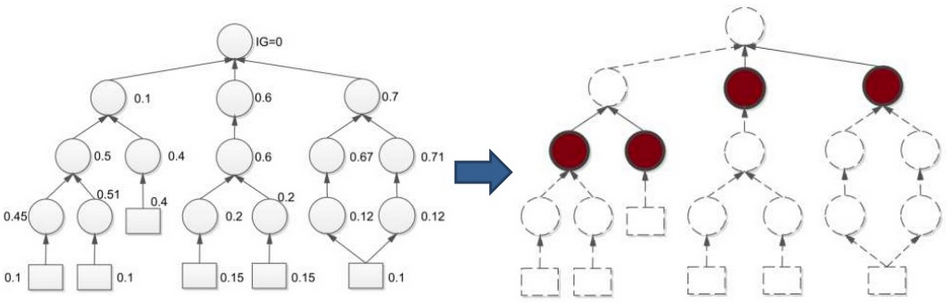
\includegraphics[width=1\linewidth]{figure/Mannheim/Opt.png}
		\label{fig:Opt}
	\end{figure}
\end{frame}
\subsection{Greedy Top Down}
\begin{frame}
	\frametitle{Greedy Top Down}
	Strategia di ricerca Greedy di tipo top down per la feature selection
	\begin{itemize}
		\item Seleziona i nodi più rappresentativi da diversi livelli della gerarchia
	\end{itemize}
	\begin{figure}[tbph]
		\centering
		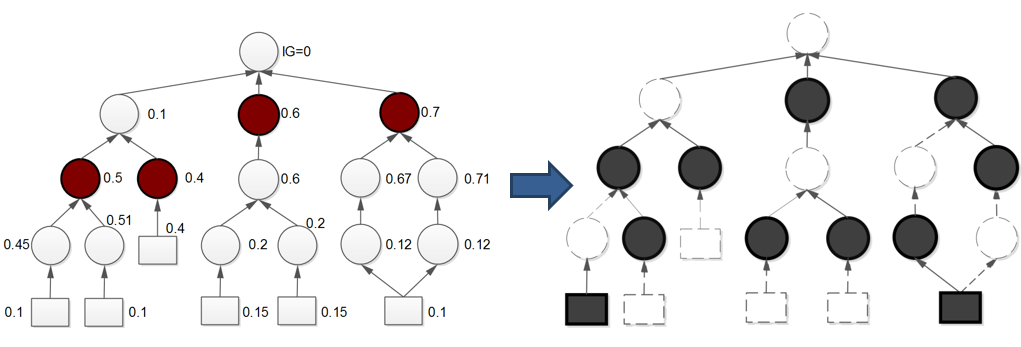
\includegraphics[width=1\linewidth]{figure/Mannheim/Greedy_Top_Down.png}
		\label{fig:GreedyTopDown}
	\end{figure}
\end{frame}

\subsection{TSEL - IG}
\begin{frame}
	\frametitle{TSEL - Information Gain}
	Tree-based feature selection tratto da \cite{jeong2013feature}
	\begin{itemize}
		\item Seleziona le feature più rappresentative da ogni ramo della gerarchia
	\end{itemize}
	\begin{figure}[tbph]
		\centering
		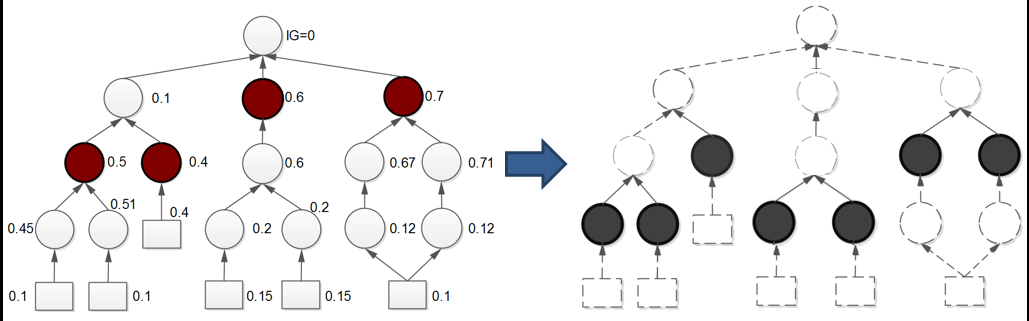
\includegraphics[width=1\linewidth]{figure/Mannheim/TSEL.png}
		\label{fig:TSEL}
	\end{figure}
\end{frame}

\subsection{SHSEL - IG}
\begin{frame}
	\frametitle{SHSEL - Information Gain \dots}
	Descritto dal paper \cite{ristoski2014feature} e nel corrispettivo sito \footnote{\url{http://goo.gl/NNlnuE}}
	\begin{itemize}
		\item The core idea of our SHSEL approach is to identify features with similar relevance, and select the most valuable abstract features, i.e. features from as high as possible levels of the hierarchy, without losing predictive power.
		\item In our approach, to measure the similarity of relevance between two nodes, we use standard correlation and information gain measure.
	\item L'approccio prevede due fasi:
	\begin{itemize}
		\item Selezione iniziale
		\item Pruning
	\end{itemize}
	\end{itemize}
\end{frame}

\begin{frame}
	\frametitle{\dots SHSEL - Information Gain \dots}
	In the first step, initial SHSEL, we are trying to identify, and filter out the ranges of nodes with similar relevance in each branch of the hierarchy
	\begin{figure}[tbph]
		\centering
		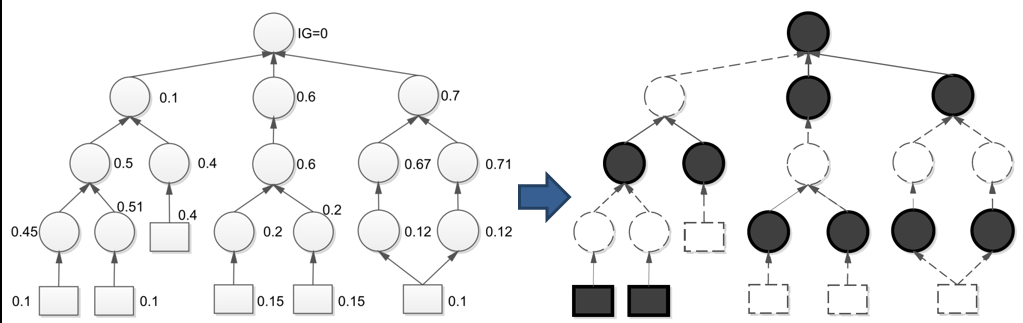
\includegraphics[width=1\linewidth]{figure/Mannheim/SHSEL_Phase1.png}
		\label{fig:SHSELPhase1}
	\end{figure}
\end{frame}

\begin{frame}
	\frametitle{\dots SHSEL - Information Gain}
	 In the second step, SHSEL Pruning, we are trying to select only the most valuable features from the previously reduced set, based on their information gain value
	\begin{figure}[tbph]
		\centering
		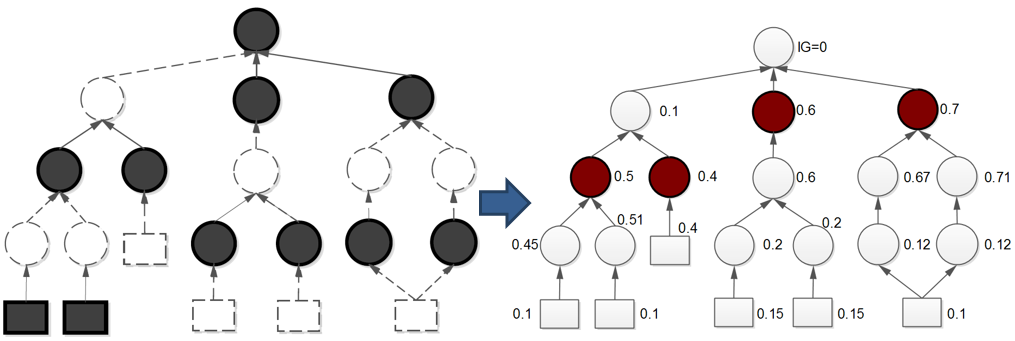
\includegraphics[width=1\linewidth]{figure/Mannheim/SHSEL_Phase2.png}
		\label{fig:SHSELPhase2}
	\end{figure}
\end{frame}
%%%%%%%%%%%%%%%%%%%%%%%%%%%%%%%%%%%%%%%%%%%%%%%%%%%%%
\begin{frame}[allowframebreaks]{Bibliography}
	\frametitle{References}
	\bibliographystyle{alpha}
	\bibliography{mybib}
\end{frame}
\end{document}
